\begin{frame}[t] \frametitle{\emph{Retrieval Augmented Generation}}
\framesubtitle{Natura dinamica dei contenuti digitali}
{\scriptsize
\onslide<1->
    \begin{minipage}[t]{\textwidth}
        \vspace*{-.5cm}
        \begin{figure}
            \centering
            \includegraphics[width=.25\textwidth]{img/RAG_1.PNG}
            \includegraphics[width=.25\textwidth]{img/RAG_2.PNG}
            $\cdots$
            \includegraphics[width=.25\textwidth]{img/RAG_4.PNG}
        \end{figure}
    \end{minipage}
    \begin{minipage}[t]{\textwidth}
        \begin{itemize}[leftmargin=10pt,align=right]
            \onslide<2->\item[\alert{\faHandORight}] Pre-addestramento costante per le LLM non è efficiente
            \onslide<3->\item[\alert{\faHandORight}] Come fare con \alert{fattoidi} (es. cariche politiche, popolazione per stato, $\ldots$)?!
        \end{itemize}
    \end{minipage}
}
\end{frame}
%
\begin{frame}[t] \frametitle{\emph{Retrieval Augmented Generation}}
{\scriptsize
\onslide<1->
\framesubtitle{Rivoluzione nel mondo dell'addestramento LLM}
\vspace*{-.5cm}
    \begin{minipage}[t]{\textwidth}
        \begin{figure}[ht]
            \centering
            \includegraphics[width=\textwidth]{img/AI-timeline-2021-2.png}
        \end{figure}
    \end{minipage}
    \onslide<1->
    \begin{minipage}[t]{.60\textwidth}
        \begin{figure}[ht]
            \centering
            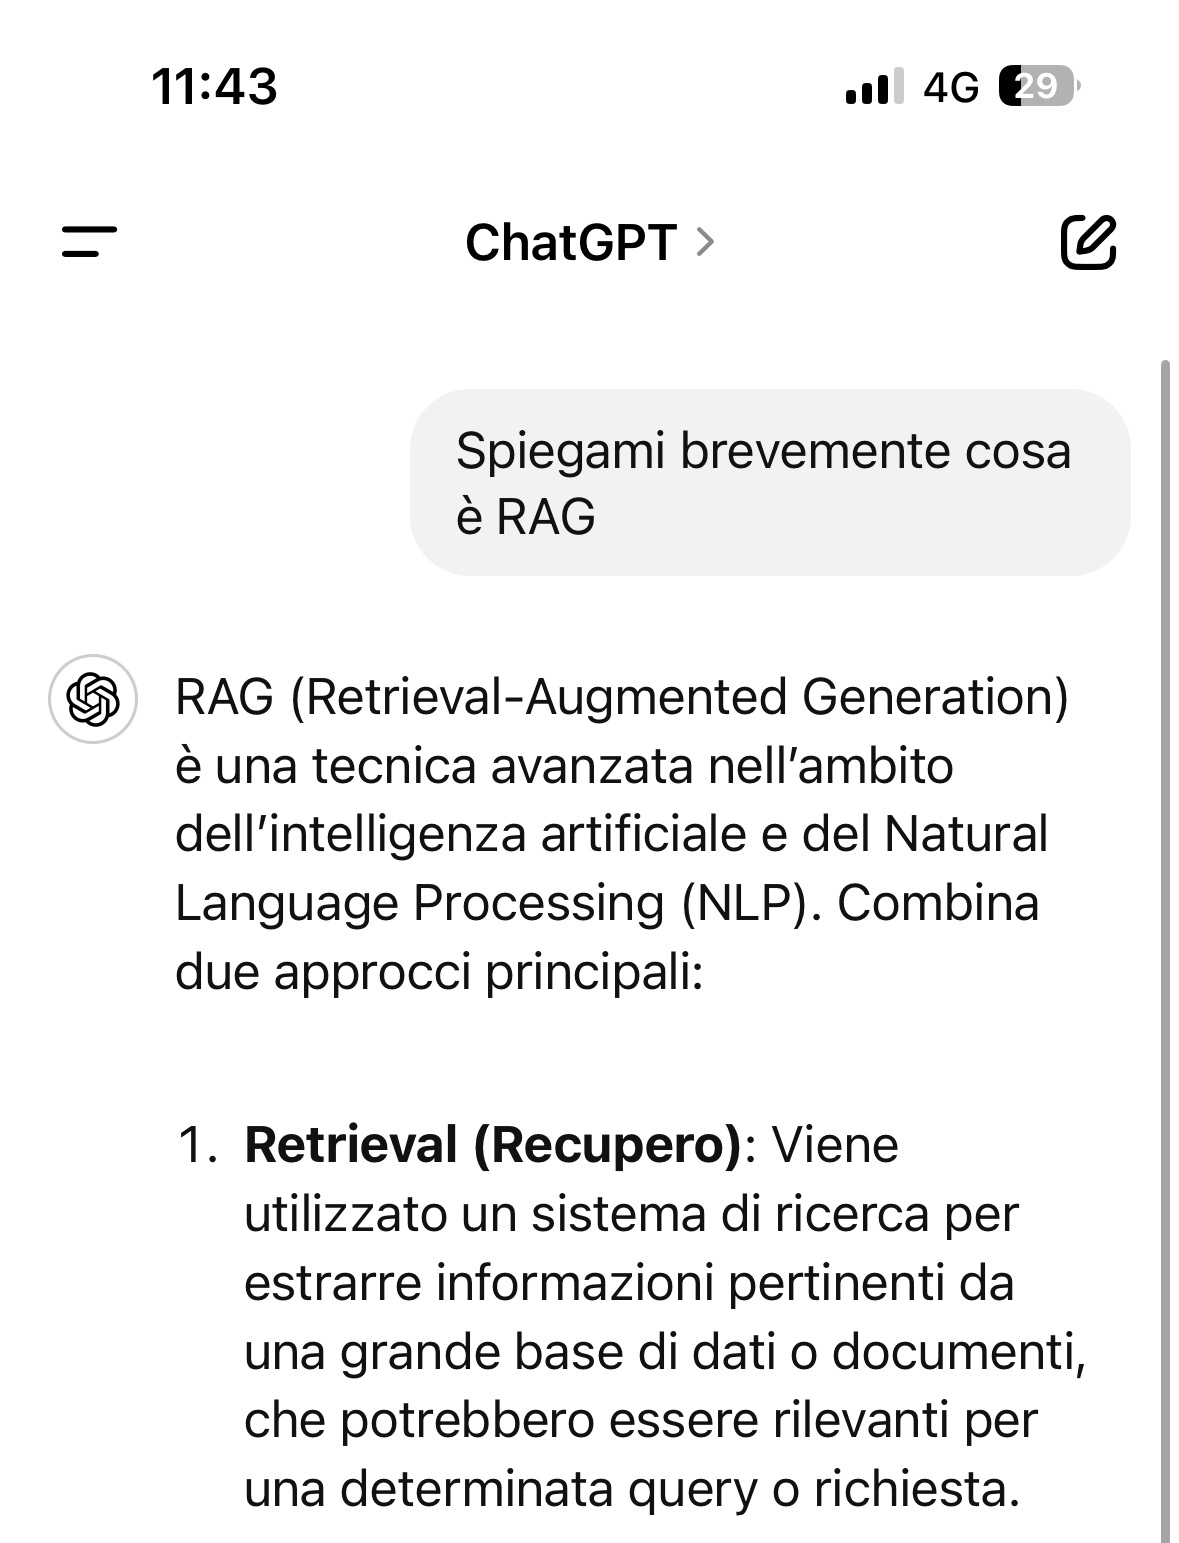
\includegraphics[width=.48\textwidth]{img/RAG_5_cut.PNG}
            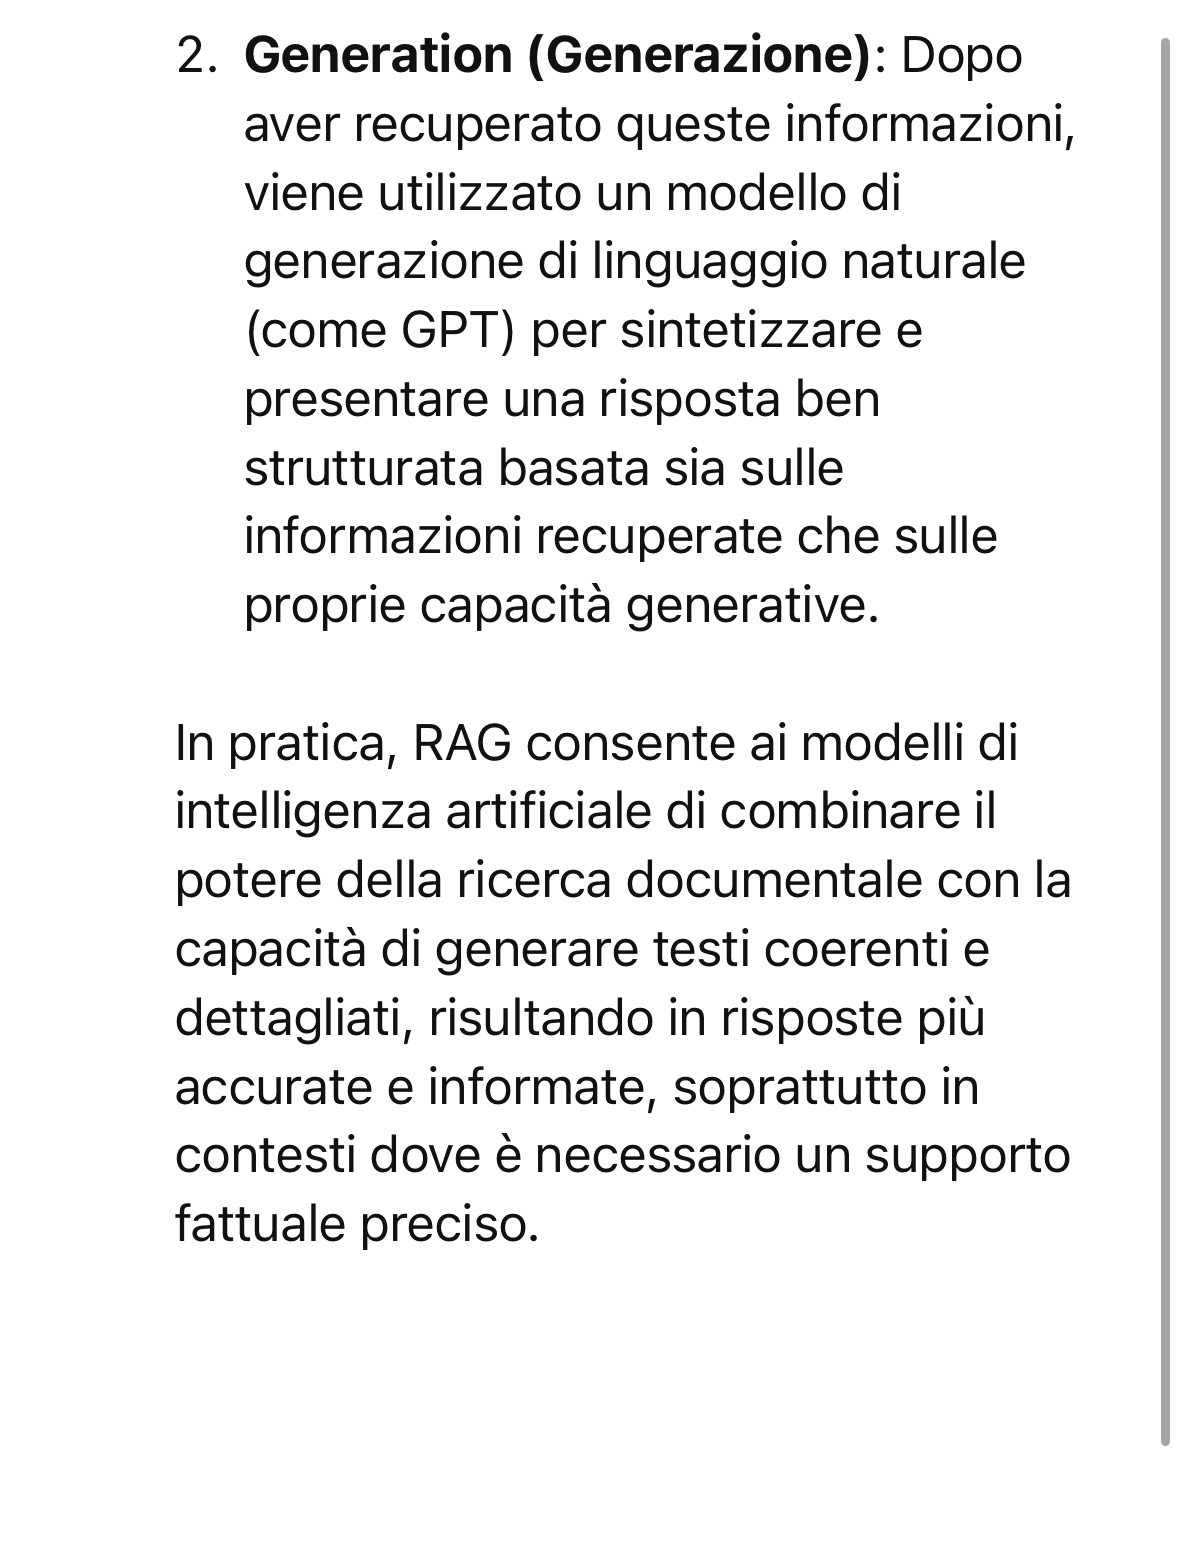
\includegraphics[width=.48\textwidth]{img/RAG_6_cut.PNG}
        \end{figure}
    \end{minipage}
    \hfill
    \begin{minipage}[t]{.35\textwidth}
        \begin{itemize}[leftmargin=10pt,align=right]
            \onslide<2->\item[\alert{\faHandORight}] Nuova frontiera del \emph{prompt engineering}
            \onslide<3->\item[\alert{\faHandORight}] Riduce i costi di addestramento LLM
            \onslide<4->\item[\alert{\faHandORight}] Mantiene costantemente aggiornati i sistemi LLM
            \onslide<5->\item[\alert{\faHandORight}] Costi di integrazione contenuti
            \onslide<6->\item[\alert{\faHandORight}] \alert{Approccio utilizzabile anche \underline{senza LLM}}
        \end{itemize}
    \end{minipage}
}
\end{frame}
%
\begin{frame}[t] \frametitle{\emph{Workflow} del processo RAG}
{\scriptsize
\only<1-2>{
    \framesubtitle{Senza LLM$\ldots$}
    \vspace*{-.3cm}
    \begin{center}
        \includegraphics[width=.75\textwidth]{img/RAG-no-LLM.png}
    \end{center}
    \begin{minipage}[t]{\textwidth}
        \vspace*{-.8cm}
        \begin{itemize}[leftmargin=10pt,align=right]
            \onslide<2->\item[\alert{\faHandORight}] Approccio \alert{non generativo}
        \end{itemize}
    \end{minipage}
}
\only<3->{
    \framesubtitle{$\ldots$ e con LLM}
    \vspace*{-.3cm}
    \begin{center}
        \includegraphics[width=.75\textwidth]{img/RAG-LLM.png}
    \end{center}
    \begin{minipage}[t]{\textwidth}
        \vspace*{-.8cm}
        \begin{itemize}[leftmargin=10pt,align=right]
            \onslide<4->\item[\alert{\faHandORight}] Approccio \alert{generativo}
        \end{itemize}
    \end{minipage}
}
}
\end{frame}
%
\begin{frame}[t] \frametitle{RAG senza LLM: esempio}
{\scriptsize
\framesubtitle{Ricerca semantica di film e serie}
\only<1>{
    \begin{center}
        \includegraphics[width=\textwidth]{img/RAG-NO-LLM-NETFLIX-0.png}
    \end{center}
}
    \only<2>{
    \begin{center}
        \includegraphics[width=\textwidth]{img/RAG-NO-LLM-NETFLIX-1.png}
    \end{center}
}
    \only<3>{
    \begin{center}
        \includegraphics[width=\textwidth]{img/RAG-NO-LLM-NETFLIX-2.png}
    \end{center}
}
    \only<4>{
    \begin{center}
        \includegraphics[width=\textwidth]{img/RAG-NO-LLM-NETFLIX-3.png}
    \end{center}
}
    \only<5>{
    \begin{center}
        \includegraphics[width=\textwidth]{img/RAG-NO-LLM-NETFLIX-4.png}
    \end{center}
}
    \only<6>{
    \begin{center}
        \includegraphics[width=\textwidth]{img/RAG-NO-LLM-NETFLIX-5.png}
    \end{center}
}
    \only<7>{
    \begin{center}
        \includegraphics[width=\textwidth]{img/RAG-NO-LLM-NETFLIX-6.png}
    \end{center}
}
}
\end{frame}
%